\PassOptionsToPackage{unicode}{hyperref}
\PassOptionsToPackage{hyphens}{url}
%
\documentclass[
]{article}
\usepackage{amsmath,amssymb}
\usepackage{iftex}
\ifPDFTeX
  \usepackage[T1]{fontenc}
  \usepackage[utf8]{inputenc}
  \usepackage{textcomp} % provide euro and other symbols
\else % if luatex or xetex
  \usepackage{unicode-math} % this also loads fontspec
  \defaultfontfeatures{Scale=MatchLowercase}
  \defaultfontfeatures[\rmfamily]{Ligatures=TeX,Scale=1}
\fi
\usepackage{lmodern}
\ifPDFTeX\else
  % xetex/luatex font selection
\fi
% Use upquote if available, for straight quotes in verbatim environments
\IfFileExists{upquote.sty}{\usepackage{upquote}}{}
\IfFileExists{microtype.sty}{% use microtype if available
  \usepackage[]{microtype}
  \UseMicrotypeSet[protrusion]{basicmath} % disable protrusion for tt fonts
}{}
\makeatletter
\@ifundefined{KOMAClassName}{% if non-KOMA class
  \IfFileExists{parskip.sty}{%
    \usepackage{parskip}
  }{% else
    \setlength{\parindent}{0pt}
    \setlength{\parskip}{6pt plus 2pt minus 1pt}}
}{% if KOMA class
  \KOMAoptions{parskip=half}}
\makeatother
\usepackage{xcolor}
\usepackage[margin=1in]{geometry}
\usepackage{color}
\usepackage{fancyvrb}
\newcommand{\VerbBar}{|}
\newcommand{\VERB}{\Verb[commandchars=\\\{\}]}
\DefineVerbatimEnvironment{Highlighting}{Verbatim}{commandchars=\\\{\}}
% Add ',fontsize=\small' for more characters per line
\usepackage{framed}
\definecolor{shadecolor}{RGB}{248,248,248}
\newenvironment{Shaded}{\begin{snugshade}}{\end{snugshade}}
\newcommand{\AlertTok}[1]{\textcolor[rgb]{0.94,0.16,0.16}{#1}}
\newcommand{\AnnotationTok}[1]{\textcolor[rgb]{0.56,0.35,0.01}{\textbf{\textit{#1}}}}
\newcommand{\AttributeTok}[1]{\textcolor[rgb]{0.13,0.29,0.53}{#1}}
\newcommand{\BaseNTok}[1]{\textcolor[rgb]{0.00,0.00,0.81}{#1}}
\newcommand{\BuiltInTok}[1]{#1}
\newcommand{\CharTok}[1]{\textcolor[rgb]{0.31,0.60,0.02}{#1}}
\newcommand{\CommentTok}[1]{\textcolor[rgb]{0.56,0.35,0.01}{\textit{#1}}}
\newcommand{\CommentVarTok}[1]{\textcolor[rgb]{0.56,0.35,0.01}{\textbf{\textit{#1}}}}
\newcommand{\ConstantTok}[1]{\textcolor[rgb]{0.56,0.35,0.01}{#1}}
\newcommand{\ControlFlowTok}[1]{\textcolor[rgb]{0.13,0.29,0.53}{\textbf{#1}}}
\newcommand{\DataTypeTok}[1]{\textcolor[rgb]{0.13,0.29,0.53}{#1}}
\newcommand{\DecValTok}[1]{\textcolor[rgb]{0.00,0.00,0.81}{#1}}
\newcommand{\DocumentationTok}[1]{\textcolor[rgb]{0.56,0.35,0.01}{\textbf{\textit{#1}}}}
\newcommand{\ErrorTok}[1]{\textcolor[rgb]{0.64,0.00,0.00}{\textbf{#1}}}
\newcommand{\ExtensionTok}[1]{#1}
\newcommand{\FloatTok}[1]{\textcolor[rgb]{0.00,0.00,0.81}{#1}}
\newcommand{\FunctionTok}[1]{\textcolor[rgb]{0.13,0.29,0.53}{\textbf{#1}}}
\newcommand{\ImportTok}[1]{#1}
\newcommand{\InformationTok}[1]{\textcolor[rgb]{0.56,0.35,0.01}{\textbf{\textit{#1}}}}
\newcommand{\KeywordTok}[1]{\textcolor[rgb]{0.13,0.29,0.53}{\textbf{#1}}}
\newcommand{\NormalTok}[1]{#1}
\newcommand{\OperatorTok}[1]{\textcolor[rgb]{0.81,0.36,0.00}{\textbf{#1}}}
\newcommand{\OtherTok}[1]{\textcolor[rgb]{0.56,0.35,0.01}{#1}}
\newcommand{\PreprocessorTok}[1]{\textcolor[rgb]{0.56,0.35,0.01}{\textit{#1}}}
\newcommand{\RegionMarkerTok}[1]{#1}
\newcommand{\SpecialCharTok}[1]{\textcolor[rgb]{0.81,0.36,0.00}{\textbf{#1}}}
\newcommand{\SpecialStringTok}[1]{\textcolor[rgb]{0.31,0.60,0.02}{#1}}
\newcommand{\StringTok}[1]{\textcolor[rgb]{0.31,0.60,0.02}{#1}}
\newcommand{\VariableTok}[1]{\textcolor[rgb]{0.00,0.00,0.00}{#1}}
\newcommand{\VerbatimStringTok}[1]{\textcolor[rgb]{0.31,0.60,0.02}{#1}}
\newcommand{\WarningTok}[1]{\textcolor[rgb]{0.56,0.35,0.01}{\textbf{\textit{#1}}}}
\usepackage{longtable,booktabs,array}
\usepackage{calc} % for calculating minipage widths
% Correct order of tables after \paragraph or \subparagraph
\usepackage{etoolbox}
\makeatletter
\patchcmd\longtable{\par}{\if@noskipsec\mbox{}\fi\par}{}{}
\makeatother
% Allow footnotes in longtable head/foot
\IfFileExists{footnotehyper.sty}{\usepackage{footnotehyper}}{\usepackage{footnote}}
\makesavenoteenv{longtable}
\usepackage{graphicx}
\makeatletter
\def\maxwidth{\ifdim\Gin@nat@width>\linewidth\linewidth\else\Gin@nat@width\fi}
\def\maxheight{\ifdim\Gin@nat@height>\textheight\textheight\else\Gin@nat@height\fi}
\makeatother
% Scale images if necessary, so that they will not overflow the page
% margins by default, and it is still possible to overwrite the defaults
% using explicit options in \includegraphics[width, height, ...]{}
\setkeys{Gin}{width=\maxwidth,height=\maxheight,keepaspectratio}
% Set default figure placement to htbp
\makeatletter
\def\fps@figure{htbp}
\makeatother
\setlength{\emergencystretch}{3em} % prevent overfull lines
\providecommand{\tightlist}{%
  \setlength{\itemsep}{0pt}\setlength{\parskip}{0pt}}
\setcounter{secnumdepth}{-\maxdimen} % remove section numbering
\usepackage{float}
\ifLuaTeX
  \usepackage{selnolig}  % disable illegal ligatures
\fi
\IfFileExists{bookmark.sty}{\usepackage{bookmark}}{\usepackage{hyperref}}
\IfFileExists{xurl.sty}{\usepackage{xurl}}{} % add URL line breaks if available
\urlstyle{same}
\hypersetup{
  pdftitle={Econometrics 2 PS4: Regression Discontinuity},
  pdfauthor={Carlos T. Estrada Arzamendi},
  hidelinks,
  pdfcreator={LaTeX via pandoc}}

\title{Econometrics 2 PS4: Regression Discontinuity}
\author{Carlos T. Estrada Arzamendi}
\date{March 21, 2024}

\begin{document}
\maketitle

\hypertarget{problem-1-sharp-regression-discontinuity}{%
\section{Problem 1: (Sharp) Regression
Discontinuity}\label{problem-1-sharp-regression-discontinuity}}



``Take any dataset with covariate X and outcome Y that are related in
some way. For instance, you can use the data on birth weight and smoking
from here: \url{http://www.stata.com/texts/eacsap/}, or any other
relevant dataset. Alternatively, feel free to simulate your own data. In
any case, please provide an explanation of your dataset. Construct a
placebo treatment by applying a rule such that Di = 1 when Xi
\textgreater= x0 for some x0. That is, modify the outcome variable Yi
for those units with Xi \textgreater= x0 by adding a constant treatment
effect, for example, add one standard deviation of the outcome plus some
noise (with mean zero). Include an explanation of what you ended up
doing''

\begin{Shaded}
\begin{Highlighting}[]
\CommentTok{\# Data Simulation}
\FunctionTok{library}\NormalTok{(truncnorm)}
\NormalTok{n }\OtherTok{=} \DecValTok{10000}

\NormalTok{data }\OtherTok{=} \FunctionTok{data.table}\NormalTok{(}
  \AttributeTok{gpa =} \FunctionTok{rtruncnorm}\NormalTok{(n, }\AttributeTok{a =} \DecValTok{0}\NormalTok{, }\AttributeTok{b =} \DecValTok{4}\NormalTok{, }\AttributeTok{mean =} \DecValTok{3}\NormalTok{, }\AttributeTok{sd =} \DecValTok{1}\NormalTok{),}
  \AttributeTok{fam\_income =} \FunctionTok{runif}\NormalTok{(n, }\AttributeTok{min =} \DecValTok{20000}\NormalTok{, }\AttributeTok{max =} \DecValTok{150000}\NormalTok{)}
\NormalTok{)}
\NormalTok{gpa\_cutoff }\OtherTok{=} \DecValTok{2}

\CommentTok{\# if gpa is below cutoff, school provides tutoring that increases score}
\NormalTok{data[, treat }\SpecialCharTok{:=} \FunctionTok{ifelse}\NormalTok{(gpa }\SpecialCharTok{\textless{}}\NormalTok{ gpa\_cutoff, }\DecValTok{1}\NormalTok{, }\DecValTok{0}\NormalTok{)]}
\NormalTok{data[, outcome\_score }\SpecialCharTok{:=}\NormalTok{ gpa}\SpecialCharTok{*}\DecValTok{300} \SpecialCharTok{+}\NormalTok{ fam\_income}\SpecialCharTok{/}\DecValTok{1000} \SpecialCharTok{+}\NormalTok{ treat}\SpecialCharTok{*}\DecValTok{200} \SpecialCharTok{+} \FunctionTok{rnorm}\NormalTok{(n, }\AttributeTok{mean =} \DecValTok{0}\NormalTok{, }\AttributeTok{sd =} \DecValTok{50}\NormalTok{)]}

\FunctionTok{datasummary\_skim}\NormalTok{(data, }\AttributeTok{out =} \StringTok{"markdown"}\NormalTok{, }\AttributeTok{title =} \StringTok{"Summary Statistics"}\NormalTok{, }\AttributeTok{histogram =}\NormalTok{ F)}
\end{Highlighting}
\end{Shaded}

\begin{longtable}[]{@{}
  >{\raggedright\arraybackslash}p{(\columnwidth - 14\tabcolsep) * \real{0.1807}}
  >{\raggedleft\arraybackslash}p{(\columnwidth - 14\tabcolsep) * \real{0.0964}}
  >{\raggedleft\arraybackslash}p{(\columnwidth - 14\tabcolsep) * \real{0.1687}}
  >{\raggedleft\arraybackslash}p{(\columnwidth - 14\tabcolsep) * \real{0.1084}}
  >{\raggedleft\arraybackslash}p{(\columnwidth - 14\tabcolsep) * \real{0.1084}}
  >{\raggedleft\arraybackslash}p{(\columnwidth - 14\tabcolsep) * \real{0.1084}}
  >{\raggedleft\arraybackslash}p{(\columnwidth - 14\tabcolsep) * \real{0.1084}}
  >{\raggedleft\arraybackslash}p{(\columnwidth - 14\tabcolsep) * \real{0.1205}}@{}}
\caption{Summary Statistics}\tabularnewline
\toprule\noalign{}
\begin{minipage}[b]{\linewidth}\raggedright
\end{minipage} & \begin{minipage}[b]{\linewidth}\raggedleft
Unique
\end{minipage} & \begin{minipage}[b]{\linewidth}\raggedleft
Missing Pct.
\end{minipage} & \begin{minipage}[b]{\linewidth}\raggedleft
Mean
\end{minipage} & \begin{minipage}[b]{\linewidth}\raggedleft
SD
\end{minipage} & \begin{minipage}[b]{\linewidth}\raggedleft
Min
\end{minipage} & \begin{minipage}[b]{\linewidth}\raggedleft
Median
\end{minipage} & \begin{minipage}[b]{\linewidth}\raggedleft
Max
\end{minipage} \\
\midrule\noalign{}
\endfirsthead
\toprule\noalign{}
\begin{minipage}[b]{\linewidth}\raggedright
\end{minipage} & \begin{minipage}[b]{\linewidth}\raggedleft
Unique
\end{minipage} & \begin{minipage}[b]{\linewidth}\raggedleft
Missing Pct.
\end{minipage} & \begin{minipage}[b]{\linewidth}\raggedleft
Mean
\end{minipage} & \begin{minipage}[b]{\linewidth}\raggedleft
SD
\end{minipage} & \begin{minipage}[b]{\linewidth}\raggedleft
Min
\end{minipage} & \begin{minipage}[b]{\linewidth}\raggedleft
Median
\end{minipage} & \begin{minipage}[b]{\linewidth}\raggedleft
Max
\end{minipage} \\
\midrule\noalign{}
\endhead
\bottomrule\noalign{}
\endlastfoot
gpa & 10000 & 0 & 2.7 & 0.8 & 0.0 & 2.8 & 4.0 \\
fam\_income & 10000 & 0 & 85409.1 & 37744.9 & 20001.0 & 85357.9 &
149973.8 \\
treat & 2 & 0 & 0.2 & 0.4 & 0.0 & 0.0 & 1.0 \\
outcome\_score & 10000 & 0 & 938.5 & 195.2 & 242.9 & 931.0 & 1464.6 \\
\end{longtable}

\hypertarget{plot-the-outcome-by-forcing-variable-the-standard-graph-showing-the-discontinuity}{%
\subsection{1.1) Plot the outcome by forcing variable (the standard
graph showing the
discontinuity)}\label{plot-the-outcome-by-forcing-variable-the-standard-graph-showing-the-discontinuity}}

\begin{Shaded}
\begin{Highlighting}[]
\CommentTok{\# Generate input data for output plot}

\NormalTok{plot1 }\OtherTok{\textless{}{-}} \FunctionTok{ggplot}\NormalTok{(data, }\FunctionTok{aes}\NormalTok{(}\AttributeTok{x =}\NormalTok{ gpa, }\AttributeTok{y =}\NormalTok{ outcome\_score, }\AttributeTok{color =} \FunctionTok{as.factor}\NormalTok{(treat), }\AttributeTok{group =} \FunctionTok{as.factor}\NormalTok{(treat))) }\SpecialCharTok{+} 
  \FunctionTok{geom\_point}\NormalTok{() }\SpecialCharTok{+}
  \CommentTok{\#geom\_smooth(aes(fill = as.factor(treat))) +}
  \FunctionTok{geom\_smooth}\NormalTok{(}\AttributeTok{method =} \StringTok{"lm"}\NormalTok{,}\AttributeTok{color =} \StringTok{"black"}\NormalTok{, }\AttributeTok{formula =}\NormalTok{ y}\SpecialCharTok{\textasciitilde{}}\NormalTok{x) }\SpecialCharTok{+} 
  \FunctionTok{labs}\NormalTok{(}\AttributeTok{x =} \StringTok{"GPA"}\NormalTok{, }\AttributeTok{y =} \StringTok{"Outcome Score"}\NormalTok{) }\SpecialCharTok{+} \FunctionTok{ggtitle}\NormalTok{(}\StringTok{"Outcome by forcing variable"}\NormalTok{) }\SpecialCharTok{+}
  \FunctionTok{geom\_vline}\NormalTok{(}\AttributeTok{xintercept =}\NormalTok{ gpa\_cutoff, }\AttributeTok{linewidth =} \DecValTok{1}\NormalTok{)}
\NormalTok{plot1}
\end{Highlighting}
\end{Shaded}

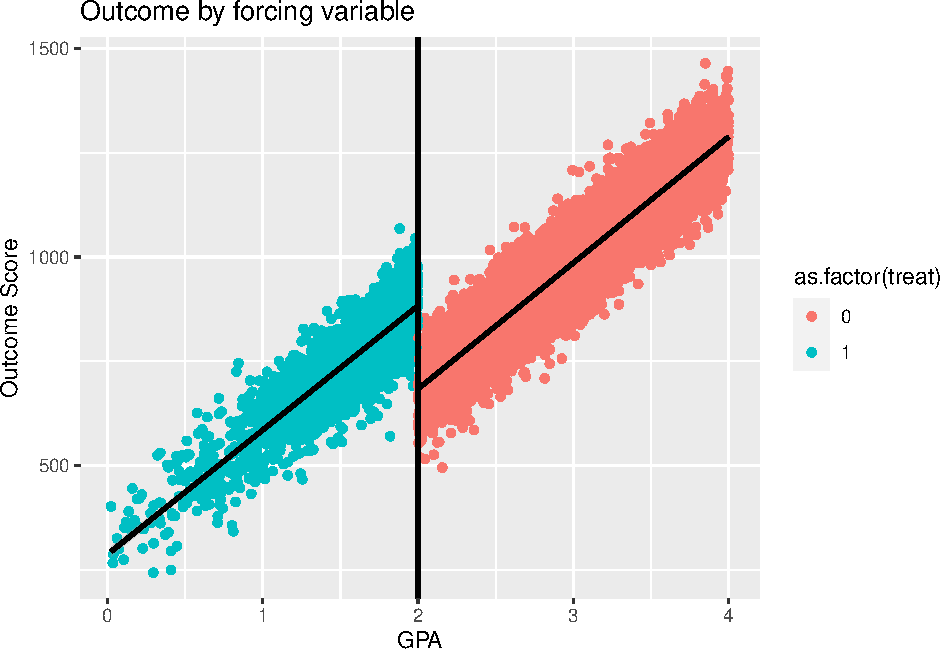
\includegraphics{EM2-PS4-Estrada_files/figure-latex/part1-1.pdf}

\hypertarget{plot-the-density-of-the-forcing-variable}{%
\subsection{1.2) Plot the density of the forcing
variable}\label{plot-the-density-of-the-forcing-variable}}

You can also embed plots, for example:

\begin{Shaded}
\begin{Highlighting}[]
\NormalTok{plot2 }\OtherTok{\textless{}{-}} \FunctionTok{ggplot}\NormalTok{(data, }\FunctionTok{aes}\NormalTok{(gpa)) }\SpecialCharTok{+} 
  \FunctionTok{geom\_histogram}\NormalTok{(}\AttributeTok{fill =} \StringTok{"blue"}\NormalTok{, }\AttributeTok{color =} \StringTok{"lightblue"}\NormalTok{, }\AttributeTok{binwidth =} \FloatTok{0.05}\NormalTok{) }\SpecialCharTok{+}
  \FunctionTok{labs}\NormalTok{(}\AttributeTok{x =} \StringTok{"GPA"}\NormalTok{, }\AttributeTok{y =} \StringTok{"Outcome Score"}\NormalTok{) }\SpecialCharTok{+} \FunctionTok{ggtitle}\NormalTok{(}\StringTok{"Density by forcing variable"}\NormalTok{) }\SpecialCharTok{+}
  \FunctionTok{geom\_vline}\NormalTok{(}\AttributeTok{xintercept =}\NormalTok{ gpa\_cutoff, }\AttributeTok{linewidth =} \DecValTok{1}\NormalTok{)}
\NormalTok{plot2}
\end{Highlighting}
\end{Shaded}

\begin{center}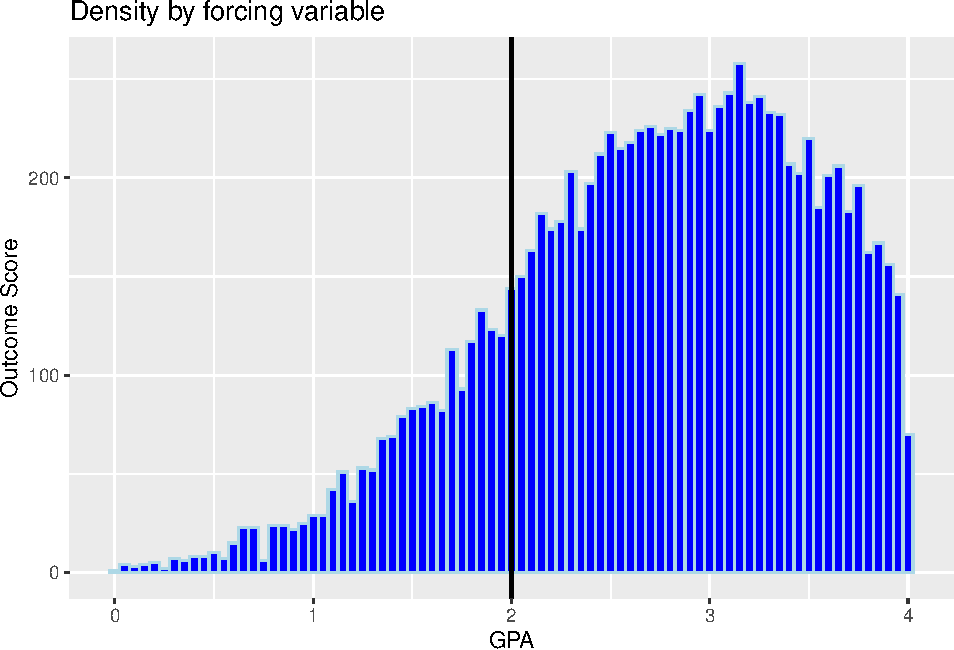
\includegraphics[width=0.75\linewidth]{EM2-PS4-Estrada_files/figure-latex/part2-1} \end{center}

\hypertarget{estimate-the-effect-using-a-local-linear-regression}{%
\subsection{1.3) Estimate the effect using a local linear
regression}\label{estimate-the-effect-using-a-local-linear-regression}}

\begin{Shaded}
\begin{Highlighting}[]
\NormalTok{reg3 }\OtherTok{=} \FunctionTok{lm}\NormalTok{(outcome\_score }\SpecialCharTok{\textasciitilde{}}\NormalTok{ treat }\SpecialCharTok{+} \FunctionTok{I}\NormalTok{(gpa}\SpecialCharTok{{-}}\NormalTok{gpa\_cutoff) }\SpecialCharTok{+} \FunctionTok{I}\NormalTok{(treat}\SpecialCharTok{*}\NormalTok{(gpa}\SpecialCharTok{{-}}\NormalTok{gpa\_cutoff)) , }\AttributeTok{data =}\NormalTok{ data)}
\FunctionTok{stargazer}\NormalTok{(reg3, }\AttributeTok{type =} \StringTok{"latex"}\NormalTok{, }\AttributeTok{title =} \StringTok{"Local Linear Regression"}\NormalTok{, }\AttributeTok{table.placement =} \StringTok{"H"}\NormalTok{,}
          \AttributeTok{header=}\ConstantTok{FALSE}\NormalTok{, }\AttributeTok{no.space =}\NormalTok{ T, }\AttributeTok{omit.stat =} \StringTok{"f"}\NormalTok{)}
\end{Highlighting}
\end{Shaded}

\begin{table}[H] \centering 
  \caption{Local Linear Regression} 
  \label{} 
\begin{tabular}{@{\extracolsep{5pt}}lc} 
\\[-1.8ex]\hline 
\hline \\[-1.8ex] 
 & \multicolumn{1}{c}{\textit{Dependent variable:}} \\ 
\cline{2-2} 
\\[-1.8ex] & outcome\_score \\ 
\hline \\[-1.8ex] 
 treat & 199.937$^{***}$ \\ 
  & (2.751) \\ 
  I(gpa - gpa\_cutoff) & 302.432$^{***}$ \\ 
  & (1.293) \\ 
  I(treat \textasteriskcentered  (gpa - gpa\_cutoff)) & $-$4.011 \\ 
  & (3.788) \\ 
  Constant & 683.559$^{***}$ \\ 
  & (1.466) \\ 
 \hline \\[-1.8ex] 
Observations & 10,000 \\ 
R$^{2}$ & 0.896 \\ 
Adjusted R$^{2}$ & 0.896 \\ 
Residual Std. Error & 62.952 (df = 9996) \\ 
\hline 
\hline \\[-1.8ex] 
\textit{Note:}  & \multicolumn{1}{r}{$^{*}$p$<$0.1; $^{**}$p$<$0.05; $^{***}$p$<$0.01} \\ 
\end{tabular} 
\end{table}

\hypertarget{estimate-the-effect-using-a-local-polynomial-of-order-2-and-3-regression}{%
\subsection{1.4) Estimate the effect using a local polynomial (of order
2 and 3)
regression}\label{estimate-the-effect-using-a-local-polynomial-of-order-2-and-3-regression}}

\begin{Shaded}
\begin{Highlighting}[]
\NormalTok{reg41 }\OtherTok{=} \FunctionTok{lm}\NormalTok{(outcome\_score }\SpecialCharTok{\textasciitilde{}}\NormalTok{ treat }\SpecialCharTok{+} \FunctionTok{I}\NormalTok{(gpa}\SpecialCharTok{{-}}\NormalTok{gpa\_cutoff) }\SpecialCharTok{+} \FunctionTok{I}\NormalTok{(treat}\SpecialCharTok{*}\NormalTok{(gpa}\SpecialCharTok{{-}}\NormalTok{gpa\_cutoff))}\SpecialCharTok{+}
             \FunctionTok{I}\NormalTok{((gpa}\SpecialCharTok{{-}}\NormalTok{gpa\_cutoff)}\SpecialCharTok{\^{}}\DecValTok{2}\NormalTok{) }\SpecialCharTok{+} \FunctionTok{I}\NormalTok{(treat}\SpecialCharTok{*}\NormalTok{(gpa}\SpecialCharTok{{-}}\NormalTok{gpa\_cutoff)}\SpecialCharTok{\^{}}\DecValTok{2}\NormalTok{), }\AttributeTok{data =}\NormalTok{ data)}
\CommentTok{\#stargazer(reg41, type = "latex", title = "Estimate Effect Using Local Polynomial of Order 2", table.placement = "H", header=FALSE, no.space = T)}
\end{Highlighting}
\end{Shaded}

\begin{Shaded}
\begin{Highlighting}[]
\NormalTok{reg42 }\OtherTok{=} \FunctionTok{lm}\NormalTok{(outcome\_score }\SpecialCharTok{\textasciitilde{}}\NormalTok{ treat }\SpecialCharTok{+} \FunctionTok{I}\NormalTok{(gpa}\SpecialCharTok{{-}}\NormalTok{gpa\_cutoff) }\SpecialCharTok{+} \FunctionTok{I}\NormalTok{(treat}\SpecialCharTok{*}\NormalTok{(gpa}\SpecialCharTok{{-}}\NormalTok{gpa\_cutoff))}\SpecialCharTok{+}
             \FunctionTok{I}\NormalTok{((gpa}\SpecialCharTok{{-}}\NormalTok{gpa\_cutoff)}\SpecialCharTok{\^{}}\DecValTok{2}\NormalTok{) }\SpecialCharTok{+} \FunctionTok{I}\NormalTok{(treat}\SpecialCharTok{*}\NormalTok{(gpa}\SpecialCharTok{{-}}\NormalTok{gpa\_cutoff)}\SpecialCharTok{\^{}}\DecValTok{2}\NormalTok{)}\SpecialCharTok{+}
             \FunctionTok{I}\NormalTok{((gpa}\SpecialCharTok{{-}}\NormalTok{gpa\_cutoff)}\SpecialCharTok{\^{}}\DecValTok{3}\NormalTok{) }\SpecialCharTok{+} \FunctionTok{I}\NormalTok{(treat}\SpecialCharTok{*}\NormalTok{(gpa}\SpecialCharTok{{-}}\NormalTok{gpa\_cutoff)}\SpecialCharTok{\^{}}\DecValTok{3}\NormalTok{), }\AttributeTok{data =}\NormalTok{ data)}
\FunctionTok{stargazer}\NormalTok{(reg3, reg41, reg42, }\AttributeTok{type =} \StringTok{"latex"}\NormalTok{, }\AttributeTok{title =} \StringTok{"Estimate Effect Using Local Polynomial of Order 2 and 3"}\NormalTok{,}
          \AttributeTok{table.placement =} \StringTok{"H"}\NormalTok{, }\AttributeTok{header=}\ConstantTok{FALSE}\NormalTok{, }\AttributeTok{no.space =}\NormalTok{ T, }\AttributeTok{omit.stat =} \StringTok{"f"}\NormalTok{)}
\end{Highlighting}
\end{Shaded}

\begin{table}[H] \centering 
  \caption{Estimate Effect Using Local Polynomial of Order 2 and 3} 
  \label{} 
\begin{tabular}{@{\extracolsep{5pt}}lccc} 
\\[-1.8ex]\hline 
\hline \\[-1.8ex] 
 & \multicolumn{3}{c}{\textit{Dependent variable:}} \\ 
\cline{2-4} 
\\[-1.8ex] & \multicolumn{3}{c}{outcome\_score} \\ 
\\[-1.8ex] & (1) & (2) & (3)\\ 
\hline \\[-1.8ex] 
 treat & 199.937$^{***}$ & 207.002$^{***}$ & 205.134$^{***}$ \\ 
  & (2.751) & (3.895) & (5.056) \\ 
  I(gpa - gpa\_cutoff) & 302.432$^{***}$ & 302.894$^{***}$ & 286.485$^{***}$ \\ 
  & (1.293) & (5.106) & (12.927) \\ 
  I(treat \textasteriskcentered  (gpa - gpa\_cutoff)) & $-$4.011 & 27.907$^{**}$ & 53.295$^{**}$ \\ 
  & (3.788) & (11.809) & (26.452) \\ 
  I((gpa - gpa\_cutoff)$\hat{\mkern6mu}$2) &  & $-$0.232 & 19.984 \\ 
  &  & (2.477) & (14.840) \\ 
  I(treat \textasteriskcentered  (gpa - gpa\_cutoff)$\hat{\mkern6mu}$2) &  & 22.565$^{***}$ & 16.930 \\ 
  &  & (7.352) & (37.061) \\ 
  I((gpa - gpa\_cutoff)$\hat{\mkern6mu}$3) &  &  & $-$6.742 \\ 
  &  &  & (4.880) \\ 
  I(treat \textasteriskcentered  (gpa - gpa\_cutoff)$\hat{\mkern6mu}$3) &  &  & 12.653 \\ 
  &  &  & (14.334) \\ 
  Constant & 683.559$^{***}$ & 683.396$^{***}$ & 686.328$^{***}$ \\ 
  & (1.466) & (2.276) & (3.112) \\ 
 \hline \\[-1.8ex] 
Observations & 10,000 & 10,000 & 10,000 \\ 
R$^{2}$ & 0.896 & 0.896 & 0.896 \\ 
Adjusted R$^{2}$ & 0.896 & 0.896 & 0.896 \\ 
Residual Std. Error & 62.952 (df = 9996) & 62.926 (df = 9994) & 62.925 (df = 9992) \\ 
\hline 
\hline \\[-1.8ex] 
\textit{Note:}  & \multicolumn{3}{r}{$^{*}$p$<$0.1; $^{**}$p$<$0.05; $^{***}$p$<$0.01} \\ 
\end{tabular} 
\end{table}

\end{document}
